% Author: Dominik Harmim <xharmi00@stud.fit.vutbr.cz>
% Author: Vojtěch Hertl <xhertl04@stud.fit.vutbr.cz>


\documentclass[a4paper, 11pt]{article}


\usepackage[czech]{babel}
\usepackage[utf8]{inputenc}
\usepackage[left=2cm, top=3cm, text={17cm, 24cm}]{geometry}
\usepackage{times}
\usepackage{graphicx}
\usepackage[unicode]{hyperref}
\usepackage[czech, boxed]{algorithm2e}


\hypersetup{
	colorlinks = true,
	hypertexnames = false,
	citecolor = red
}


\begin{document}
	%%%%%%%%%%%%%%%%%%%%%%%%%%%%%%%% Titulní stránka %%%%%%%%%%%%%%%%%%%%%%%%%%%
	\begin{titlepage}
		\begin{center}
			
\includegraphics[width=0.77\linewidth]{inc/FIT_logo.pdf} \\

			\vspace{\stretch{0.382}}

			\Huge{Simulační studie} \\
			\LARGE{\textbf{Rozvoz jídla firmou Freshbox}} \\
			\Large{Tým: ModelX} \\
			\Large{Varianta 2: Doprava zboží nebo osob}

			\vspace{\stretch{0.618}}
		\end{center}

		\begin{minipage}{0.5 \textwidth}
			{\Large \today}
		\end{minipage}
		\hfill
		\begin{minipage}[r]{0.5 \textwidth}
			\Large
			\begin{tabular}{l l}
				\textbf{Dominik Harmim} & \textbf{(xharmi00)} \\
				Vojtěch Hertl & (xhertl04) \\
			\end{tabular}
		\end{minipage}
	\end{titlepage}



	%%%%%%%%%%%%%%%%%%%%%%%%%%%%%%%% Obsah %%%%%%%%%%%%%%%%%%%%%%%%%%%%%%%%%%%%%
	\pagenumbering{roman}
	\setcounter{page}{1}
	\tableofcontents
	\clearpage



	%%%%%%%%%%%%%%%%%%%%%%%%%%%%%%%% Úvod %%%%%%%%%%%%%%%%%%%%%%%%%%%%%%%%%%%%%%
	\pagenumbering{arabic}
	\setcounter{page}{1}

	\section{Úvod}

	V~této práci je řešen proces sestavování modelu \cite[snímek 7]{IMS_slides}
	pro rozvoz jídla po Brně firmou Freshbox \cite{Freshbox} a~jeho následná
	simulace \cite[snímek 33]{IMS_slides}. Díky tomuto modelu a~simulačním
	experimentům \cite[snímek 9]{IMS_slides} nad ním je možno pozorovat
	efektivitu a~přínos v~různých podmínkách. Smyslem experimentů je zjistit,
	jak kvalitně navržený je systém \cite[snímek 18]{IMS_slides} a~zda by se
	změnou některého z~ovlivňujících faktorů mohl zdokonalit. V~reálném
	systému může být obtížné a~finančně nákladné tyto ovlivňující faktory
	měnit a~zjišťovat, jak se bude systém chovat, proto je vhodné získat
	nové znalosti o~reálném systému použitím principů modelování
	a~simulace \cite[snímek 9]{IMS_slides}.


	\subsection{Autoři, zdroje}

	Projekt vypracovali studenti Dominik Harmim a~Vojtěch Hertl z~FIT VUT
	v~Brně.

	K~technické části této práce bylo využito zdrojů z~kursu Modelování
	a~simulace na FIT VUT v~Brně. Jako zdroj k~faktům sloužily webové stránky
	firmy Freshbox a~také vedoucí této firmy, Mgr. Silvie Obadalová\\
	(\texttt{obadalova@freshbox.cz}).


	\subsection{Ověření validity}

	Ověřování validity \cite[snímek 37]{Freshbox} probíhalo telefonicky
	a~elektronicky s~vedoucí firmy Freshox, magistrou Obadalovou. Na základě
	této komunikace byla získána všechna data potřebná k~experimentálnímu
	ověřování validity modelu. Statistická data byla extrahována z~naměřených
	statistik firmy Freshbox. Validita byla také ověřena pomocí experimentů
	a~srovnáním s~realitou.



	%%%%%%%%%%%%%%%% Rozbor tématu a použitých metod/technologií %%%%%%%%%%%%%%%
	\section{Rozbor tématu a~použitých metod/technologií}

	Všechna použitá fakta jsou zprůměrována ze všech získaných informací. \\

	Zákazníci mají předem objednaná jidla od firmy Freshbox, která tato jídla
	každý den od 6:30 hodin do 12:30 hodin (tj. 6 hodin) rozváží zákazníkům po
	Brně a~okolí. Firma Freshbox rozváží jidlo 16 auty, přičemž jedno auto
	je schopné naložit maximálně 500 jídel. Každý den se rozváží
	průměrně 21\,200 jídel $\pm$~1\,000 jídel. Firma má na začátku rozvozu
	již všechna jídla připravena a~v~6:30 hodin se připraví všechna auta,
	do kterých se naloží maximální počet jídel, který je dán maximální
	kapacitou auta. Naložení jednoho auta průměrně trvá 11 minut
	$\pm$~3 minuty. Rozvoz všech jídel jednoho auta trvá průměrně 97 minut
	$\pm$~12 minut. Při tomto rozvozu každé auto urazí průměrně 43 km
	$\pm$ 8 km. Pro rozvoz se požívají auta Volkswagen Caddy 1.9 TDI.
	Tato auta mají spotřebu
	7,7\,l/100\,km\footnote{\url{https://www.auto-data.net/en/volkswagen-caddy-maxi-life-typ-2k-1.9-tdi-105hp-8855}}
	nafty při městském provozu. Když auto rozveze všechna
	naložená jídla, vrátí se na pobočku Freshbox, aby se mohla naložit další
	jídla. Samotné nakládání jídel provádí sám řadič daného auta. Tento proces
	se opakuje tak dlouho, dokud nejsou rozvezena všechna jídla. Jeden zákazník
	(právnická nebo fyzická osoba) si samozřejmě může objednat více jídel na
	jedno místo doručení, což se typicky děje, protože pravidelnými zákazníky
	jsou firmy, které si objednávají denně řádově desítky jídel.


	\subsection{Použité postupy}

	Pro vytvoření modelu byl použit programovací jazyk C++ za podpory
	simulační knihovny SIMLIB \cite{SIMLIB}. Tyto technologie jsou ideální pro
	řešení zadaného problému, jelikož poskytují všechna potřebná rozhraní
	k~implementaci modelu. Další výhodou je, že se jedná o~otevřený software,
	jsou to multi-platformní technologie a~poměrně jednuduše se používají,
	nejedná se o~nic zbytečně těžkopádného. Dále byly použity postupy popsané
	v~textech ke kursu Modelování a simulace na FIT VUT v~Brně \cite{IMS_slides}
	k~vytváření Petriho sítě \cite[snímek 123]{IMS_slides} a~samotnému
	programování za použití knihovny SIMLIB.


	\subsection{Popis původu použitých metod/technologií}

	Použili jsme standardní třídy a~funkce jazyka
	C++\footnote{\url{https://cppreference.com/w/cpp}}.
	Drželi jsme se standardu C++14. Využívali jsme monžosti oběktově
	orientovaného návrhu.

	Pro překlad zdrojových souborů byly použity nástroje
	CMake\footnote{\url{https://cmake.org}}
	a~GNU Make\footnote{\url{https://www.gnu.org/software/make}}.

	Knihovna SIMLIB byla získána z~oficálních stránek tohoto
	nástroje\footnote{\url{http://www.fit.vutbr.cz/~peringer/SIMLIB}}.
	Použili jsme nejnovější dostupnou verzi (ke dni \today), tj 3.07.
	Autory tohoto nástroje jsou Petr Peringer, David Leska a David Martinek,
	viz \cite{SIMLIB}. Pro účely vytvoření našeho simulačního modelu
	\cite[snímek 44]{IMS_slides} jsme používali standardní nástroje
	a~rohraní této knihovny.



	%%%%%%%%%%%%%%%%%%%%%%%%%%%%%%%% Koncepce modelu %%%%%%%%%%%%%%%%%%%%%%%%%%%
	\section{Koncepce modelu}

	V~této sekci se zpracovává návrh konceptuálního (abstraktního) modelu
	\cite[snímek 48]{IMS_slides} nad systémem, který je brán ze své podstaty
	jako systém hromadné obsluhy \cite[snímek 136]{IMS_slides}. Při vytváření
	je potřeba vybrat ze všech údajů ty podstatné informace pro model.
	Z~rozboru tématu plyne, že je důležité namodelovat všecho, co souvisí se
	samotným rozvozem. Díky skutečnosti, že všechny jednotlivé údaje jsou
	zprůměrovány, je zapotřebí simulovat průběh jednoho dne, přičemž se
	samozřejmě může den ode dne nepatrně lišit.	Na oba proměnné časové údaje
	při modelování se tedy použije rovnoměrné rozdělení
	\cite[snímek 89]{IMS_slides} s~vyhovující odchylkou. Aby se model
	zjednodušil, průměrný počet jídel, který se každý den rozváží, se
	zaokrouhlí, aby byl dělitelný maximální kapacitou aut. Na validitu to má
	nepatrný vliv, až zanedbatelný, jelikož jsou údaje zprůměrovány. Dále
	značka auta, spotřeba paliva a~cena nejsou pro model důležitá, tyto
	informace budou použity při zefektivňování systému. Přesto, že tato
	situace reálně často, díky již nabraným zkušenostem z~reality, nenastává,
	pro lepší experimentování je přidán druhý koncový stav, který znamená,
	že směna skončí dříve než jsou rozvezena všechna jídla, tedy nějaká
	jídla zbydou na skladě. Tento stav značí neúspěšné dokončení směny,
	protože se nestihlo rozvést všechno jídlo v časovém limitu. Předpokládá se
	také, že auto, které započne ještě během pracovní směny svůj cyklus, ho
	celý dokončí. Ovšem pokud mezitím skončila směna, znamená to, že byl
	rozvoz neúspěšný z~časového hlediska.


	\subsection{Popis konceptuálního modelu}
	\label{section:conceptual_model_desc}

	Model, viz příloha \ref{appendix:petri_net}, se skládá ze~dvou hlavních
	větví. První značí samotný průběh rozvozu jídel a~druhá časovač. Druhá
	z~větví jen určuje, jak dlouho probíhá pracovní směna, to je 6 hodin,
	a~jakmile směna skončí, skončí rozvoz jídel. První větev má dvě vstupní
	proměnné -- počet aut a~počet jídel. Auto zde slouží jako obslužná linka,
	kde pokud je některé volné a~připravené na rozvoz a~zároveň jsou ještě
	nějaká jídla na skladě, začnou se nakládat. Pokud ale již byla všechna
	jídla rozvezena a~všechna auta jsou připravena na rozvoz, skončí pracovní
	směna. Po naložení jídel se auto vydá na cestu a~všechna jídla rozveze.
	Po ukončení této činnosti je auto zase volné a~připraveno k~dalšímu použití.


	\subsection{Forma konceptuálního modelu}

	Model je vizualizován pomocí Petriho sítě v~příloze
	\ref{appendix:petri_net} a~doplněn informacemi a~legendou.



	%%%%%%%%%%%%%%%%%%% Architektura simulačního modelu %%%%%%%%%%%%%%%%%%%%%%%%
	\section{Architektura simulačního modelu}

	Při spuštění simulačního modelu \cite[snímek 44]{IMS_slides} se spustí
	jednotlivé simulační experimenty, jeden po druhém, viz kapitola
	\ref{sectiion:experiments}. Simulační model je možné, po jeho přeložení
	příkazem \texttt{make}, spustit příkazem \texttt{make run}. Po dokončení
	běhu simulace se na standardní výstup vypíší informace o~provedených
	experimentech. Před začátkem každého z~experimentů se vypíše modelový
	čas \cite[snímek 21]{IMS_slides} začátku experimentu, počet dostupných
	aut pro rozvážení jídla a~počet jídla, které je potřeba rozvézst. Na
	konci každého z~experimentů se vypíše modelový čas konce experimentu,
	počet jídel, které se nestihly rozvést, celková auty ujetá vzdálenost,
	celková spotřeba pohonných hmot všech aut, informace o~skladu
	\cite[snímek 184]{IMS_slides} aut a~statistiky ohledně času nakládání aut,
	době trvání rozvozu jídel, ujeté vzdálenosti a~spotřebě aut.

	Před spuštěním každého z~experimentů se inicializuje modelový čas tak, aby
	doba trvání experimentu odpovídala jednomu dni v~reálném čase
	\cite[snímek 21]{IMS_slides}, protože modelujeme jeden den rozvozu jídla.
	Jedna časová jednotka modelového času odpovídá jedné minutě v~reálném
	čase.

	Spuštění experimentu v~simulačním modelu znamená vytvořit a~aktivovat
	proces \cite[snímek 121]{IMS_slides}, který reprezentuje pracovní směnu
	a~následně spustit samotnou simulaci. Tento proces reprezentující
	pracovní směnu lze vytvořit s~parametry, které mění chování simulace.
	Tyto parametry jsou měněny při spouštění jednotlivých experimentů. Jedná
	se o~parametr značící počet aut pro rozvoz jídel, samotný počet jídel
	a~odchylku o~této hodnoty.

	Na algoritmu \ref{algorithm:workshift} je znázorněno chování procesu
	pracovní směny a~na algoritmu \ref{algorithm:car} je znázorněno chování
	procesu auta.\\

	\begin{algorithm}[H]
		\caption{Chování procesu pracovní směny}
		\label{algorithm:workshift}
		\SetKw{Break}{break}

		vytvoření události reprezentující časovač, který po určité době
		ukoční směnu\;
		\While{jsou na skladě jídla připravena k rozvozu}
		{
			čekání na volné auto a~jeho zabrání\;
			\eIf{na skladě už nejsou žádná jídla}
			{
				vrácení auta do skladu aut\;
				\Break\;
			}
			{
				odebrání jídel ze skladu, které budou naloženy do auta\;
				vytvoření a~aktivavce procesu auta\;
			}
		}
		čekání, až budou všechna auta ve skladu\;
		ukončení směny\;
	\end{algorithm}

	\begin{algorithm}[H]
		\caption{Chování procesu auta}
		\label{algorithm:car}

		čekání na naložení auta\;
		čekání na rozvezení všech jídel\;
		vrácení auta do skladu aut\;
	\end{algorithm}


	\subsection{Mapování konceptuálního modulu do simulačního modelu}

	Jak je popsáno v~kapitole \ref{section:conceptual_model_desc}
	a~znázorněno v~Petriho síťi v příloze \ref{appendix:petri_net}, časovač,
	který ukončí směnu po uplynutí konce směny, je v simulačním modelu
	implementován jako událost \cite[snímek 169]{IMS_slides}, která
	při jejím vytvoření naplánuje sama sebe na čas, kdy má pracovní směna
	skončit. V~popisu chování této události je potom implementováno
	ukončení procesu pracovní směny. Této události v~simulačním modelu
	odpovídá třída \texttt{WorkShiftTimer}.

	Pracovní směna je v~simulačním modelu implementována jako proces, který
	při svém vytvoření vytvoří a~inicializuje sklad
	\cite[snímek 184]{IMS_slides} aut a~sdílenou proměnnou, která reprezentuje
	momentální počet jídel pro rozvoz. Chování tohoto procesu
	je znázorněno algoritmem \ref{algorithm:workshift}. Tomuto procesu
	v~simulačním modelu odpovídá třída \texttt{WorkShift}.

	Rozvoz jídla auty je v~simulačním modelu implementováno procesem, jehož
	chování je znázorněno na algoritmu \ref{algorithm:car}. Tomuto process
	v~simulačním moodelu odpovídá třída \texttt{Car}.



	%%%%%%%%%%%%%%% Podstata simulačních experimentů a jejich průběh %%%%%%%%%%%
	\section{Podstata simulačních experimentů a~jejich průběh}

	Cílem experimentů bylo nejdříve ověřit validitu modelu, případně zpětně
	upravit vstupní průměrné hodnoty, aby byl model co nejpodobnější skutečnosti.
	Další podstatou experimentů bylo demonstrovat, jak je systém efektivní,
	zjistit jeho limity a pokusit se o optimalizaci. Pomocí posledního
	experimentu se zjišťovalo, jestli je možné bez ohledu na režii systém
	rozšířit a urychlit pracovní směnu.


	\subsection{Postup experimentování}

	Každý experiment spočíval ve spuštění simulace 5krát po sobě v cyklu se
	zvolenými hodnotami. Všechny podstatné výstupní údaje se poté vložily do
	tabulky a zprůměrovaly. V každém experimentu také probíhala kontrola
	úspěšnosti, tedy zda se stihlo rozvést všechno jídlo během směny. Pokud
	směna skončila v momentě, kdy bylo alespoň 1 auto na cestě, experiment se
	označil za neúspěch. Pokud není stoprocentní úspěšnost, nelze počítat,
	že je experiment validní a celý se považuje za neúspěšný. Nakonec se z
	výsledků učiní závěr a pokud nebyl experiment úspěšný, jsou na základě
	těchto dat zvoleny nové vstupní hodnoty pro další experiment.

	\begin{enumerate}
		\item Určení vstupních hodnot, podle zadání experimentu.

		\item Spuštění simulace.

		\item Vypsání výstupů do tabulky.

		\item Zprůměrování výsledku, zhodnocení a učinění závěru.

	\end{enumerate}


	\subsection{Experimenty}
	\label{sectiion:experiments}

	\subsubsection{Experiment 1}

	První experiment má za úkol ověřit validitu modelu. Používá reálné hodnoty,
	které byly získány při zjišťování informací. Průměrný počet jídel je tedy
	21200 a počet aut 16. Spuštěn byl jen jednou.

	\begin{table}[h!]
		\centering
		\begin{tabular}{|r|r|r|r|r|r|}
			\hline
			\multicolumn{6}{|l|}{\textbf{Experiment 1}}   \\ \hline
			 Počet jídel & Počet aut & Celkový čas & Ujetá vzdálenost [km] & Spotřeba [l] & \textbf{Úspěch} \\ \hline
			 21400 & 16 & 5:36 & 1831 & 140,9 & \textbf{100\%} \\ \hline
		\end{tabular}
	\end{table}

	Z tabulky je zřejmé, že je model validní. Celkový čas nedosahuje nikdy
	6 hodin, rozvoz má dokonce průměrně 14 minut rezervu.

	\subsubsection{Experiment 2}

	Cílem druhého experimentu bylo zjistit limity systému ve smyslu, kolik
	jídel je za aktuálních podmínek firma schopná rozvézt za jednu směnu.
	Vstupní hodnota "počet jídel" byla tedy při každém novém experimentu
	zvýšena o určitou hodnotu.

	\begin{table}[h!]
		\centering
		\begin{tabular}{|r|r|r|r|r|}
			\hline
			\multicolumn{5}{|l|}{\textbf{Experiment 2}}   \\ \hline
			 Počet jídel & Počet aut & Celkový čas & \textbf{Úspěch} & \textbf{Průměrný počet jídel} \\ \hline
			 21400 & 16 & 5:36 & \textbf{100\%} & \textbf{21200} \\ \hline
			 23400 & 16 & 5:39 & \textbf{100\%} & \textbf{23000} \\ \hline
			 24500 & 16 & 5:57 & \textbf{20\%}  & \textbf{24200} \\ \hline
		\end{tabular}
	\end{table}

	Při použití průmerného počtu jídel 23000 byla úspěšnost rozvozu ještě
	stoprocentní, ale při zvýšení této hodnoty o dalších 1200 už z 80\%
	pokusů doba směny dosáhla na hodnotu 6 hodin a některá auta stále ještě
	rozvážela. Z experimentů vyplynulo, že při překročení hranice 24000 jídel
	nebylo téměř možné stihnout rovoz v časovém intervalu.

	\subsubsection{Experiment 3}

	V tomto experimentu je záměr zjistit díky změně počtu aut, zda se nedá
	snížit spotřeba paliva a tím snížit režii. Postupným odebíráním nebo
	přidáváním rozvážejících aut se bude ujetá vzálenost a spotřeba měnit.

	\begin{table}[h!]
		\centering
		\begin{tabular}{|r|r|r|r|r|r|}
			\hline
			\multicolumn{6}{|l|}{\textbf{Experiment 3}}   \\ \hline
			 Počet jídel & \textbf{Počet aut} & Celkový čas & Ujetá vzdálenost [km] & \textbf{Spotřeba [l]} & \textbf{Úspěch} \\ \hline
			 21400 & \textbf{16} & 5:36 & 1831 & \textbf{140,9} & \textbf{100\%} \\ \hline
			 21400 & \textbf{15} & 5:44 & 1836 & \textbf{141,3} & \textbf{100\%} \\ \hline
			 21400 & \textbf{14} & 5:57 & 1801 & \textbf{138,6} & \textbf{40\%}  \\ \hline
			 21400 & \textbf{17} & 5:30 & 1839 & \textbf{141,6} & \textbf{100\%} \\ \hline
			 21400 & \textbf{25} & 3:47 & 1837 & \textbf{141,4} & \textbf{100\%} \\ \hline
		\end{tabular}
	\end{table}

	Tento experiment vrací neočekávané výsledky. Při změně počtu aut, pokud je
	úspěšnost storprocentní, se vzdálenost a tedy i spotřeba liší jen nepatrně.
	Je zřejmé, že čím více by se udělalo pokusů, tím více by si byly hodnoty podobné.
	Lze tedy usoudit, že spotřeba není závislá na počtu aut, ale spíše na počtu
	rozvážených jídel.

	\subsubsection{Experiment 4}

	Díky poslednímu experimentu je snaha dojít k závěru, jestli systém ustojí
	i při větších číslech. Zvýšení počtu průměrně rozvážených jídel na 40000 a
	zároveň požadavek zrychení rozvozu o hodinu, takže maximální přípustný čas
	je 5 hodin. Proměná bude počet aut, nezáleží na ceně.

	\begin{table}[h!]
		\centering
		\begin{tabular}{|r|r|r|r|r|r|}
			\hline
			\multicolumn{6}{|l|}{\textbf{Experiment 4}}   \\ \hline
			 Počet jídel & \textbf{Počet aut} & \textbf{Celkový čas} & Ujetá vzdálenost [km] & Spotřeba [l] & \textbf{Úspěch (5h)} \\ \hline
			 39700 & \textbf{40} & \textbf{4:34} & 3417 & 263,1 & \textbf{60\%}  \\ \hline
			 39700 & \textbf{42} & \textbf{3:50} & 3397 & 262,2 & \textbf{100\%} \\ \hline
		\end{tabular}
	\end{table}

	Už po dvou experimentech se podařilo dosáhnout stoprocentní úspěšnosti. Při
	40 autech byly nějaké pokusy neúspěšné, ale při 42 autech se stihla všechna
	jídla rozvézt průměrně za 3 hodiny a 50 minut, což je dokonce o hodinu rychleji
	než bylo požadováno.


	\subsection{Závěry experimentů}

	Bylo provedeno více než 9 experimentů v různých podmínkách. V průběhu experimentování
	byla zjištěna validita původního modelu. Díky dalším experimentům se podařilo zjistit
	několik užitečných informací. Experimenty lze považovat s dostatečnou věrohodností za
	správný zdroj informací, neboť se každý experiment skládal z několika pokusů, z nichž
	byly všechny výsledky ještě zprůměrovány.



	%%%%%%%%%%%%%%%%% Shrnutí simulačních experimentů a závěr %%%%%%%%%%%%%%%%%%
	\section{Shrnutí simulačních experimentů a~závěr}



	%%%%%%%%%%%%%%%%%%%%%%%%%%%%%%%% Citace %%%%%%%%%%%%%%%%%%%%%%%%%%%%%%%%%%%%
	\clearpage
	\bibliographystyle{czechiso}
	\renewcommand{\refname}{Literatura}
	\bibliography{documentation}



	%%%%%%%%%%%%%%%%%%%%%%%%%%%%%%%% Přílohy %%%%%%%%%%%%%%%%%%%%%%%%%%%%%%%%%%%
	\clearpage
	\appendix

	\section{Petriho síť}
	\label{appendix:petri_net}
	\begin{figure}[!ht]
		\centering
		\vspace{-1.2cm}
		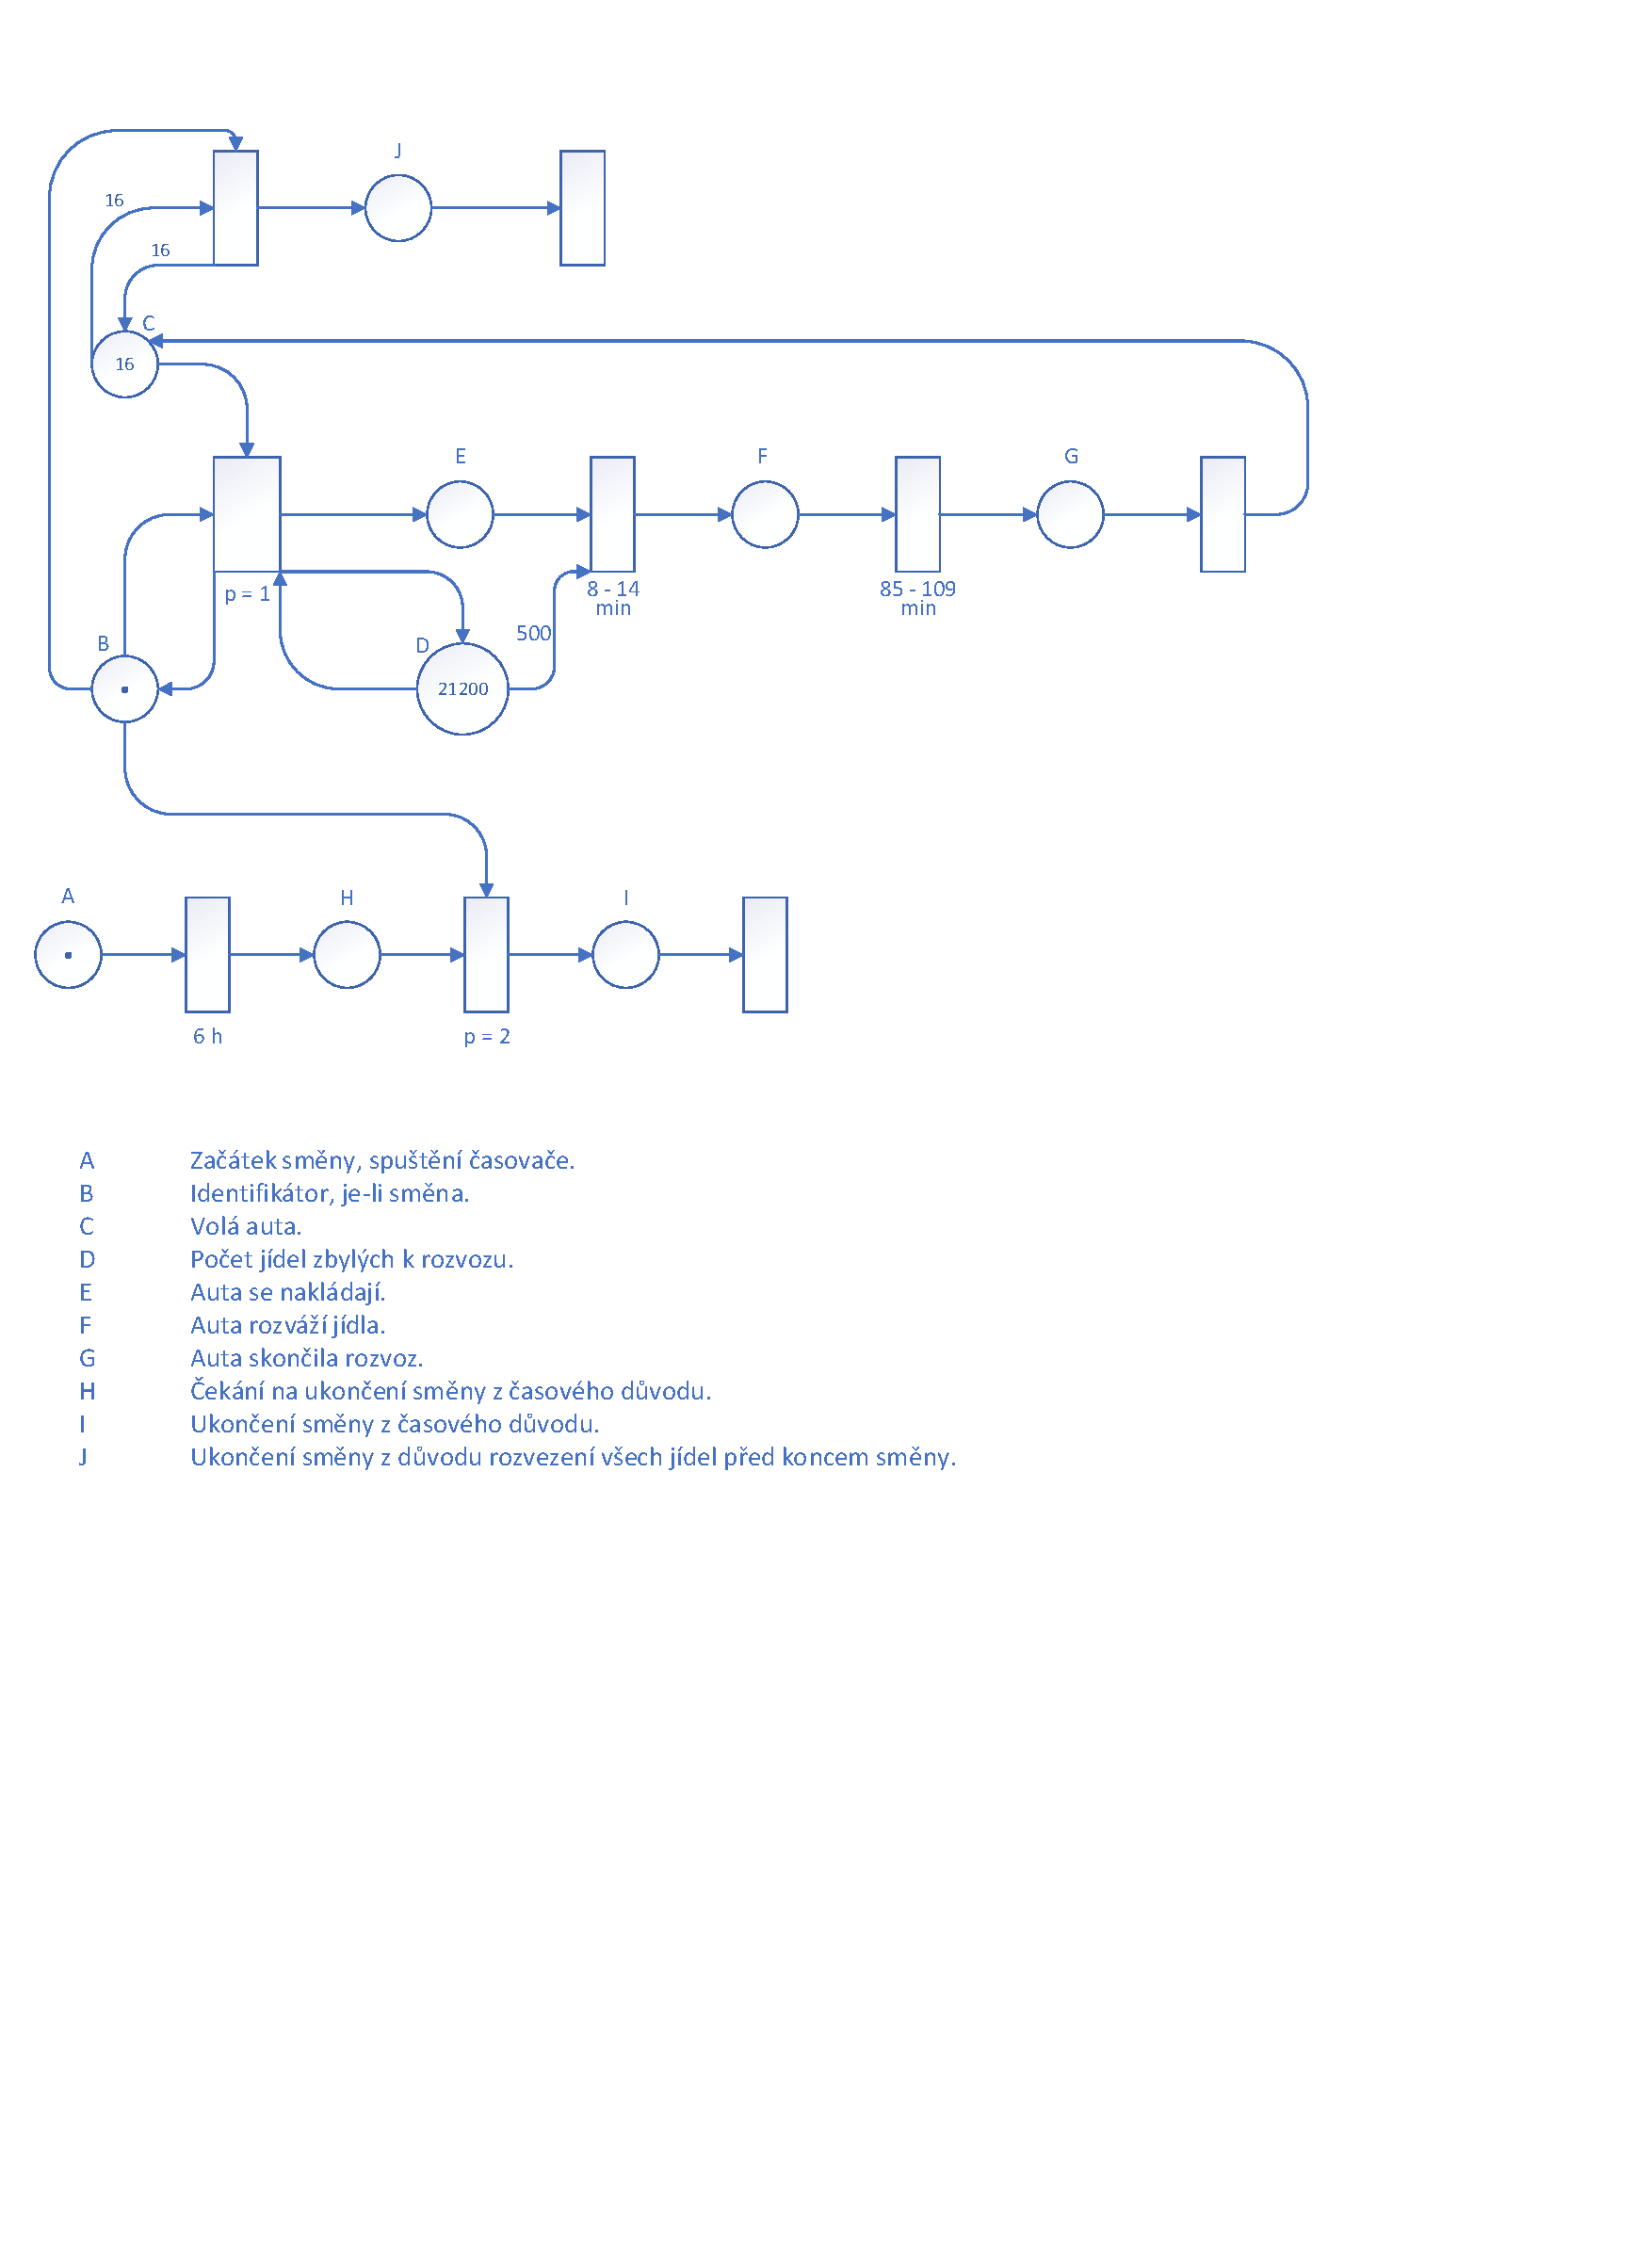
\includegraphics[width=0.95\linewidth]{inc/petri_net.pdf}
		\caption{Petriho síť}
		\label{figure:petri_net}
	\end{figure}
\end{document}
